%%%%%%%%%%%%%%%%%%%%%%%%%%%%%%%%%%%%%%%%%%%%%
% ELO 2,3,5,6
% Planning for Detailed Design

% Chapter 4: Detailed Design

% System Diagram with functional blocks 

% 4.1 Detailed design of component 1
% I chose to use a Mongo database instead of {x,y,z} because of ...
% List technical details

% 4.2 Detailed design of component 2

% 4.3 Detailed design of component 3

% 4.4 Detailed design of component 4v
%%%%%%%%%%%%%%%%%%%%%%%%%%%%%%%%%%%%%%%%%%%%%

\chapter{Low-Level System Design} 
\label{Detailed_design}

\section{Program Flow}
\begin{figure}[H]
    \centering
    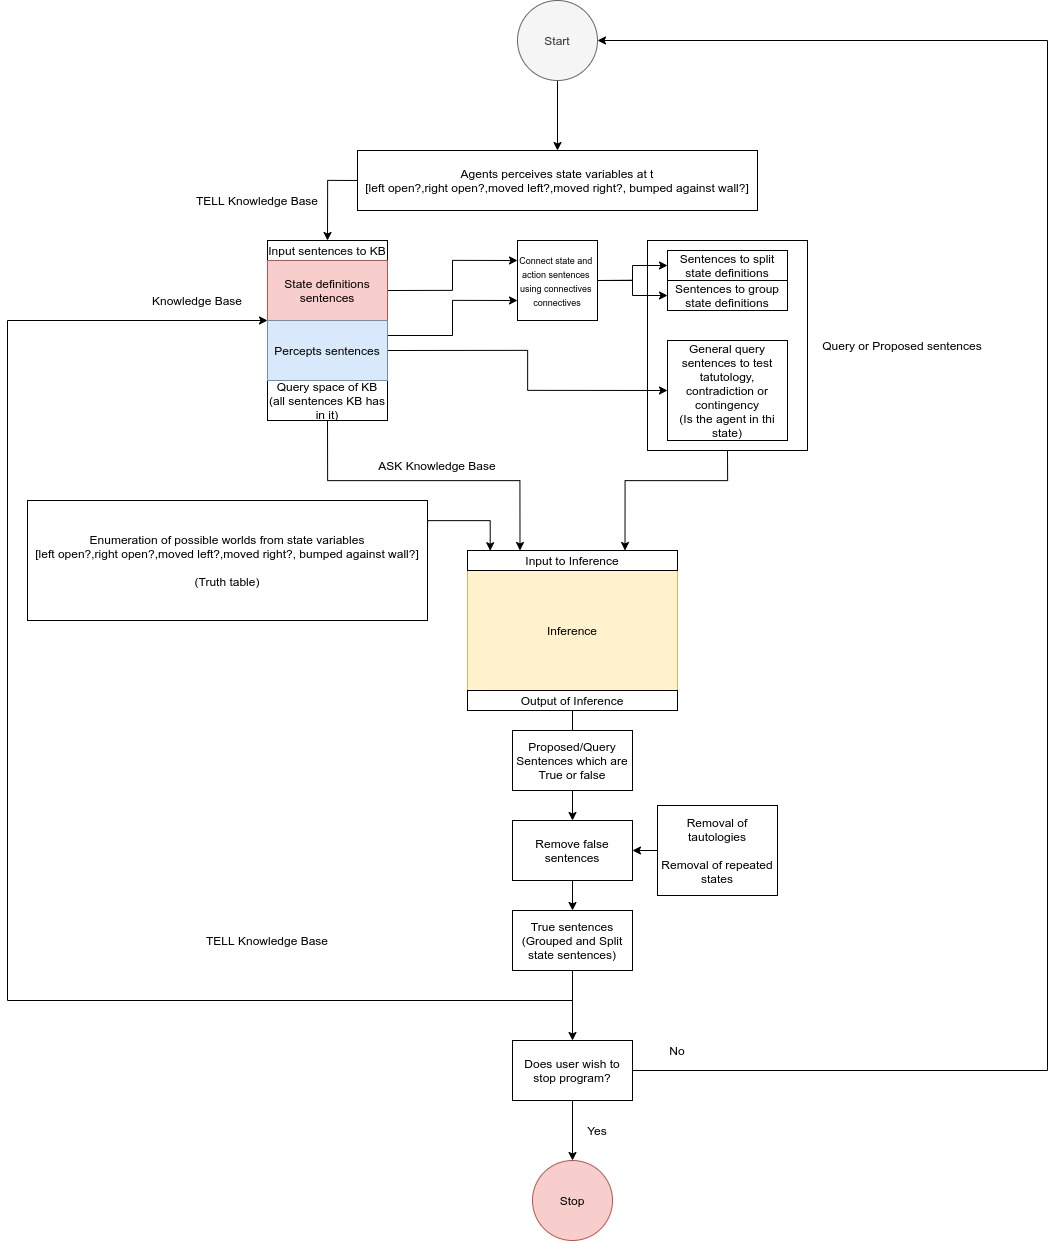
\includegraphics[scale=.3]{Figures/new_program_flow.jpg}
    \caption{Program Flow for full system} 
    \label{fig:program_flow}
\end{figure}

\section{Knowledge Base Agent}

The agent only receives percepts as inputs and action as outputs to map a representation of the environment. Thus, a percept vector (equation \ref{eq:percept_vector}) and action vector (equation \ref{eq:action_vector}) was defined. We also define a state vector (equation \ref{eq:state_vector}) using these vectors.


\begin{subequations}
\begin{align}
    \mathbf{P_t}=
\begin{bmatrix}
L_t & R_t & U_t & UL_t & UR_t & B_t & BL_t & BR_t
\end{bmatrix} 
 \label{eq:percept_vector}\\
\mathbf{A_t}=
\begin{bmatrix}
ML_t & MR_t & MU_t & MD_t & MB_t 
\end{bmatrix} 
 \label{eq:action_vector}\\
       \mathbf{S_t}=
\begin{bmatrix}
P_t & A_t  
\end{bmatrix}
 \label{eq:state_vector}
\end{align}
\end{subequations}


\section{Detailed Sub-Systems Descriptions}
\subsection{Environment}
\subsection{Knowledge Base}
\subsection{Inference Procedure}
\section{Learning Algorithms} 
\section{Forming Groups of States}
\subsection{Split State Definitions Using AND}
\subsection{Merge State Definitions Using OR}
%\citep{Discrete_Maths}
\newpage
